\begin{spacing}{1.5}
\phantom
\phantom
\phantom
\phantom
\section{Research Design}
\phantom
\phantom
To overcome the problems found in previous analyses (\emph{Chapter 2.4}), this study will improve on Ward and Tithecott's (1993) research design in several ways. \\

\noindent Miyanishi and Johnson (2001:1464) argued that any comparison between the numbers of fires between the Extensive and Intensive fire management zones cannot be valid due to a difference in fire detection resolution (see \emph{Chapter 2.2.1}). However, no such difference exists between the Intensive and Measured zones, due to the fact that all fires in both the Intensive and Measured zones are actioned and, therefore, recorded whether suppressed or not. \\

\noindent For a comparison to be made however, each zone needs to employ a different fire management strategy. In this case the fire management strategy employed after Initial Attack has failed (i.e., fires that grow >3 \emph{ha}) does in fact differ to a significant degree. In the Intensive zone, all fires that escape Initial Attack, continue to be aggressively attacked until extinguished. Whereas, in the Measured zone, escaped fires are assessed on a cost--benefit analysis, as to whether fire suppression should continue (Hirsch \emph{et al}. 1998). It can be said therefore, that the 'aggressiveness' of continued fire suppression  employed to fight escaped fires in the Intensive zone is, to some unknown degree, likely to be greater than that being employed in the Measured zone. Given this simple proposition, one could hypothosis that, on average, more escaped fires would be suppressed in the Intensive zone, than in the Measured zone. However, if the opposite is found to be true, the effectiveness of continued suppression must be in doubt. \\

\noindent As such, testing this hypothosis should provide evidence as to whether continued suppression has been effective (using Cumming's definition of 'effectiveness', see \emph{Chapter 2.3}).

\subsection{Hypotheses}
Given that our definition of effective fire suppression requires that the observed proportion of large fires in areas with aggressive suppression be lower than in those areas without (\emph{Chapter 2.3}), the following hypotheses were developed: \\

\noindent $H_{\mathrm{0}}$ $\Leftarrow$ Null hypothesis: that the proportion of large fires is independent of the fire suppression strategy being employed. \\

\noindent $H_{\mathrm{S}}$ $\Leftarrow$ Strategy hypothesis: that the proportion of large fires is dependent on the fire suppression strategy being employed$\ast$. \\

\noindent $\ast$ With the proportion of large fires expected to be lower in the Intensive zone than the Measured zone, if fire suppression is effective. \\

Operationalising these hypotheses will require a value to signify when continued suppression can said to have failed. For this, I decided to classify fires that burn more than 200 hectares as having 'escaped' continued suppression (i.e., have failed to be suppressed). While somewhat arbitrary, Cumming (2005:2) suggests that it is at this point where such fires become highly distructive events, as fires this large are thought to account for the vast majority (up to 96\%) of the area burned by forest fires every year (Strauss \emph{et al}. 1989:319; Johnson \emph{et al}. 2001). Preventing fires from crossing this threshold, therefore, is a primary concern for fire managers in Ontario and was also the main focus of Ward and Tithecott's (1993) original analysis.

\subsection{Materials and Sources}

The analysis will use annual fire statistics over the period 1989--2004, derived from provincial fire management records in the Ontario Ministry of Natural Resources (OMNR) forest fire database (retrieved \texttt{18 Feb 2012}). This database is an archive of all fires detected and reported to the provincial aviation and forest fire management centre. Over the study period, the OMNR received 22461 such reports. Each report includes the following variables: The year of each fire (\texttt{FIRE\_YEAR}); The fire management zone in which the fire was found (\texttt{FIRE\_MGT\_ZONE}); If known, the cause of the fire, i.e., lightening or anthropogenic (\texttt{GENERAL\_CAUSE}); The fire's size, measured in hectares (\texttt{FINAL\_SIZE}); and both the Latitude and Longitude of the fire's location (\texttt{LATITUDE, LONGITUDE}).

\subsection{Experimental Conditions}

As discussed in \emph{Chapter 2.3.3}, variation in a multitude of  environmental factors could be competing causal elements in the distribution of forest fires between each fire management zone (in addition to the fire management strategy employed). As such, these environmental factors must be controlled for under scientific experimental conditions.

\subsubsection{Spatial Variation}

The delineation required to control for spatial variation in forest fire distributions will be achieved by sub--dividing the dataset into several 'ecoregions'. These ecoregion classifications are commonly used by fire managers at the Ministry of Natural Resources as a way of categorising areas in Ontario based on ecological factors (OMNR 2007: Perera \emph{et al}. 2009). The system used to create these classifications is called the Ecological Land Classification (ELC) system, which is based on Angus Hills' (1959) original classifications, that were first developed in the 1950s. Since that time, the Ministry of Natural Resources has refined Ontario's ecological regions to be compatible with both national and international classification systems (OMNR 2007). \\

\begin{figure}[h]
  \centering
    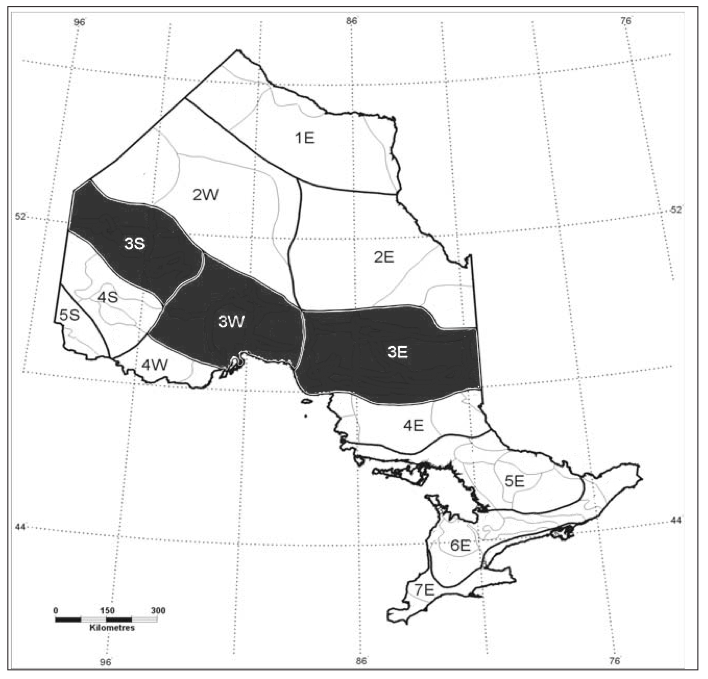
\includegraphics[width=.85\textwidth]{media/fig6}
      \caption[Ontario's ecoregions 3E, 3W, and 3S]{\emph{Ontario's ecoregions 3E, 3W, and 3S (Adapted from Perera \emph{et al}. 1998:12).}}
        \label{fig6}
\end{figure}

\noindent Each ecoregion is defined by a characteristic range and pattern in the following variables (OMNR 2007:4):

\begin{itemize}
  \item Geology
  \item Climate (temperature, precipitation, humidity)
  \item Physiography (soils, slope, aspect)
  \item Vegetation (species, biodiversity)\\
\end{itemize}

\noindent While Ontario is subdivided into a total of 14 of these ecoregions, only 3 have been chosen to be studied (3E, 3W, and 3S), due to the availability of relevant data (see \emph{Figure~\ref{fig6}}, on page~\pageref{fig6}). Given that ecoregion 2 is covered solely by the Extensive zone and ecoregions 4 and 5 covered solely by the Intensive fire management zone, a comparison between fires in the Measured and Intensive zones is not possible within these regions, and therefore, were excluded from this study. In addition, ecoregions 1, 6 and 7 are not subject to forest fire management at all, and therefore, were not applicable to this research.\\

\noindent Despite these limitations, the study area is still highly representative of the boreal forests under active fire management in Ontario (covering approximately 50\% of the forested area). The majority of the study area is Crown Land (i.e., government owned) and is managed extensively for timber (Perera \emph{et al}. 2009:2). The relative forest covers are as follows:

\begin{itemize}
  \item \textbf{3E} -- 3,541,098 ha (53.5\% of total area)
  \item \textbf{3W} -- 7,417,259 ha (83.6\% of total area)
  \item \textbf{3S} -- 12,926,327 ha (94.5\% of total area) 
\end{itemize}

\subsubsection{Humidity and Fire Frequency}

As mentioned in Chapter 2, Ontario's forests exhibit longitudinal gradients in environmental variables associated with forest fire dynamics. Fortunately, sub--setting the dataset into the three ecoregions will also allow for the analysis to account for these variations, given that the 3 ecoregions selected cover the whole province from East to West ($48\,^{\circ}$-- $52\,^{\circ}$N and $79\,^{\circ}$-- $95\,^{\circ}$W), (Beverly and Martell 2005; Suffling 1995). While ecoregion 4S has the highest rate of forest fires in Ontario, it is only covered by the Intensive zone (as one would expect), therefore, could not be included in this analysis (Ashiq 2011:13). \\

\noindent The 3 ecoregions also represent a full range of humidity in the region (Ashiq 2011:13). According to Hills' (1959) classifications, the area under study conforms largely to three distinct regions of humidity as follows:

\begin{itemize}
  \item \textbf{3E} -- Medium Humid
  \item \textbf{3W} -- Dry Humid
  \item \textbf{3S} -- Sub Humid \\
\end{itemize}

\noindent These classification are however, general approximations. According to Ashiq (2011:13), the very Southern part of ecoregion 3S for example, is thought to have a similar climate to 3W (the driest and most fire prone region under study) and therefore experiences similar fire patterns. Analysing such fine spatial variations is however, beyond the scope of this study. What is known, however, is that ecoregion 3W experiences more fires than 3S, due to differences in humidity.

\subsubsection{Temporal Variation}

As mentioned in \emph{Chapter 2.2.4}, the Boreal forests of Canada are known to exhibit a high annual variation in the area burned by forest fires. Cumming (2005) has argued that this inter--annual variation can potentially confound fire suppression efforts. This is because fire managers do not have an infinite amount of fire fighting resources with which to attack new forest fires. Therefore, on days with high numbers of forest fires, the effectiveness of suppression is bound to be limited (given that fire fighters can only attack so many fires simultaneously). Cumming (2005:776) found that the annual number of fires (annual arrival counts), were strongly correlated with the daily load (i.e., the number of fires, fire fighters have to attack simultaneously), and thus, he suggests these statistics can be used as a proxy in determining any effect the variation in fire load may have on the effectiveness of fire suppression. As such, the effect of temporal variation can be controlled for in the statistical analysis (detailed in \emph{Chapter 4:Methodology}).

\subsubsection{Data Error}

Podur et al. (2003) and Turner (2009) have both found data points in the OMNR dataset to be erroneous. Their analysis of the dataset shows some fires having started over lakes and rivers, which is clearly impossible. The authors concluded that the source of such error is likely to caused by the relative coarseness of the records. Often, individual fire locations are only recorded to nearest minute. From which, rounding errors can displace a fire's original location by up to 1 km (Turner 2009:203). Fortunately, given the time and distance scale at which this study is operating these types of error will not have a significant affect on the results.

\subsection{Reproducibility}
As Vitek and Kalibera (2011:36) point out, the confirmation of results by independent researchers is ``at the core of the scientific method''. However, additional research confirming the results of scientific investigations is usually based only on the information presented in the publication itself. Errors in analysis can often be traced back to the point at which data presented in a paper becomes detached from the operation used to produce that data in the first place. Therefore, while reproducibility is an enviable minimum standard, full replication (i.e., that the original data and code used for analysis is available) is now considered the gold standard in Science (see \emph{Figure~\ref{fig8}}). \\

\begin{figure}[h!]
  \centering
    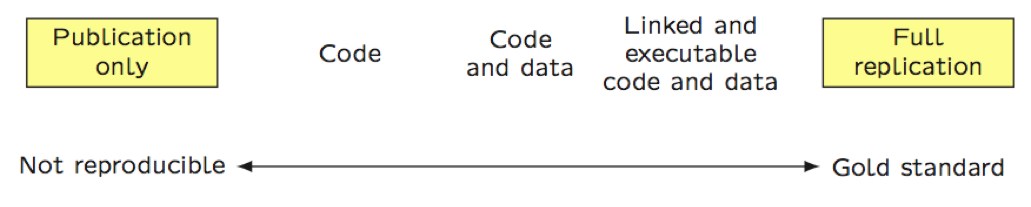
\includegraphics[width=.85\textwidth]{media/fig8}
      \caption[The Reproducibility Spectrum]{\emph{The Reproducibility Spectrum (adapted from Peng 2011).}}
        \label{fig8}
\end{figure}

\noindent Full replication is better than simply being reproducible, as having the exact code with which the experiment was performed, allows other researchers to easily uncover errors (or fraud). To achieve this gold standard, researchers must fulfil the following requirements (adapted from Schwab \emph{et al}. 2000):

\begin{itemize}
  \item \textbf{Data:} All datasets used in the analysis are made available.
  \item \textbf{Methods:} All computer code underlying the results, figures and tables is made available, and ideally the program required to execute that code is also freely available and open source.
  \item \textbf{Documentation:} The computer code must be documented to a sufficient standard that others are able to repeat the analysis.
  \item \textbf{Distribution:} All of the above must be distributed as openly as possible.
\end{itemize}

\noindent This research will employ all the recommendations outlined above. To do so, all analysis will be carryed out using statistical programming, rather than a propriety statistics application (such as SPSS, STATA etc...) and simply reporting the results in the text. The R system for statistical computation (R Development Core Team 2004) and the R-Studio Integrated Development Environment (R--Studio Development Team 2011) were used throughout. In addition, Sweave (Leisch 2002) will be used to include all of the R code necessary to replicate the analysis within the .Rnw version of this file. \\ 

\noindent The results presented in this paper therefore, are not simply reported, but calculated inline. This means that there is complete transparency in how the results were analysed, leaving no room to manipulate the figures in support of one particular hypothesis over another. This method of analysis is an example of what is known as 'literate programming' which simply means that the all the data and code necessary for producing the results are contained within the document itself (Gentleman and Lang 2007).\\

\noindent To aid with the dissemination of this resource, the R code of the project will be uploaded to the author's github repository (\texttt{https://github.com/craigrshento\linebreak n/masters\_thesis}) and distributed under the creative commons licence.
\end{spacing}
\clearpage
